\section{Climate Data Cleaning and Missing Value Treatment}\label{subsec:climate_cleaning}

\subsection{Identification of Missing Values}

\begin{figure}[H]
\centering
\begin{minipage}[t]{0.55\textwidth}
\raggedright
\vspace{0pt}

All three climate datasets contain a small but non-negligible proportion of missing values:
\begin{itemize}
    \item Precipitation: 0.28\% missing,
    \item Maximum temperature: 0.28\% missing,
    \item Minimum temperature: 0.28\% missing.
\end{itemize}

Crucially, missing entries occur on the \emph{same spatial cells} across all three variables, as verified by identical \texttt{cell\_id} sets. Spatial visualization of missing precipitation values (Figure~\ref{fig:missing_spatial}) shows that these gaps are concentrated along the perimeter of the Area of Interest, indicating edge effects caused by raster clipping and grid intersection rather than true data absence.
\end{minipage}
\hfill
\begin{minipage}[t]{0.4\textwidth}
\centering
\vspace{0pt}
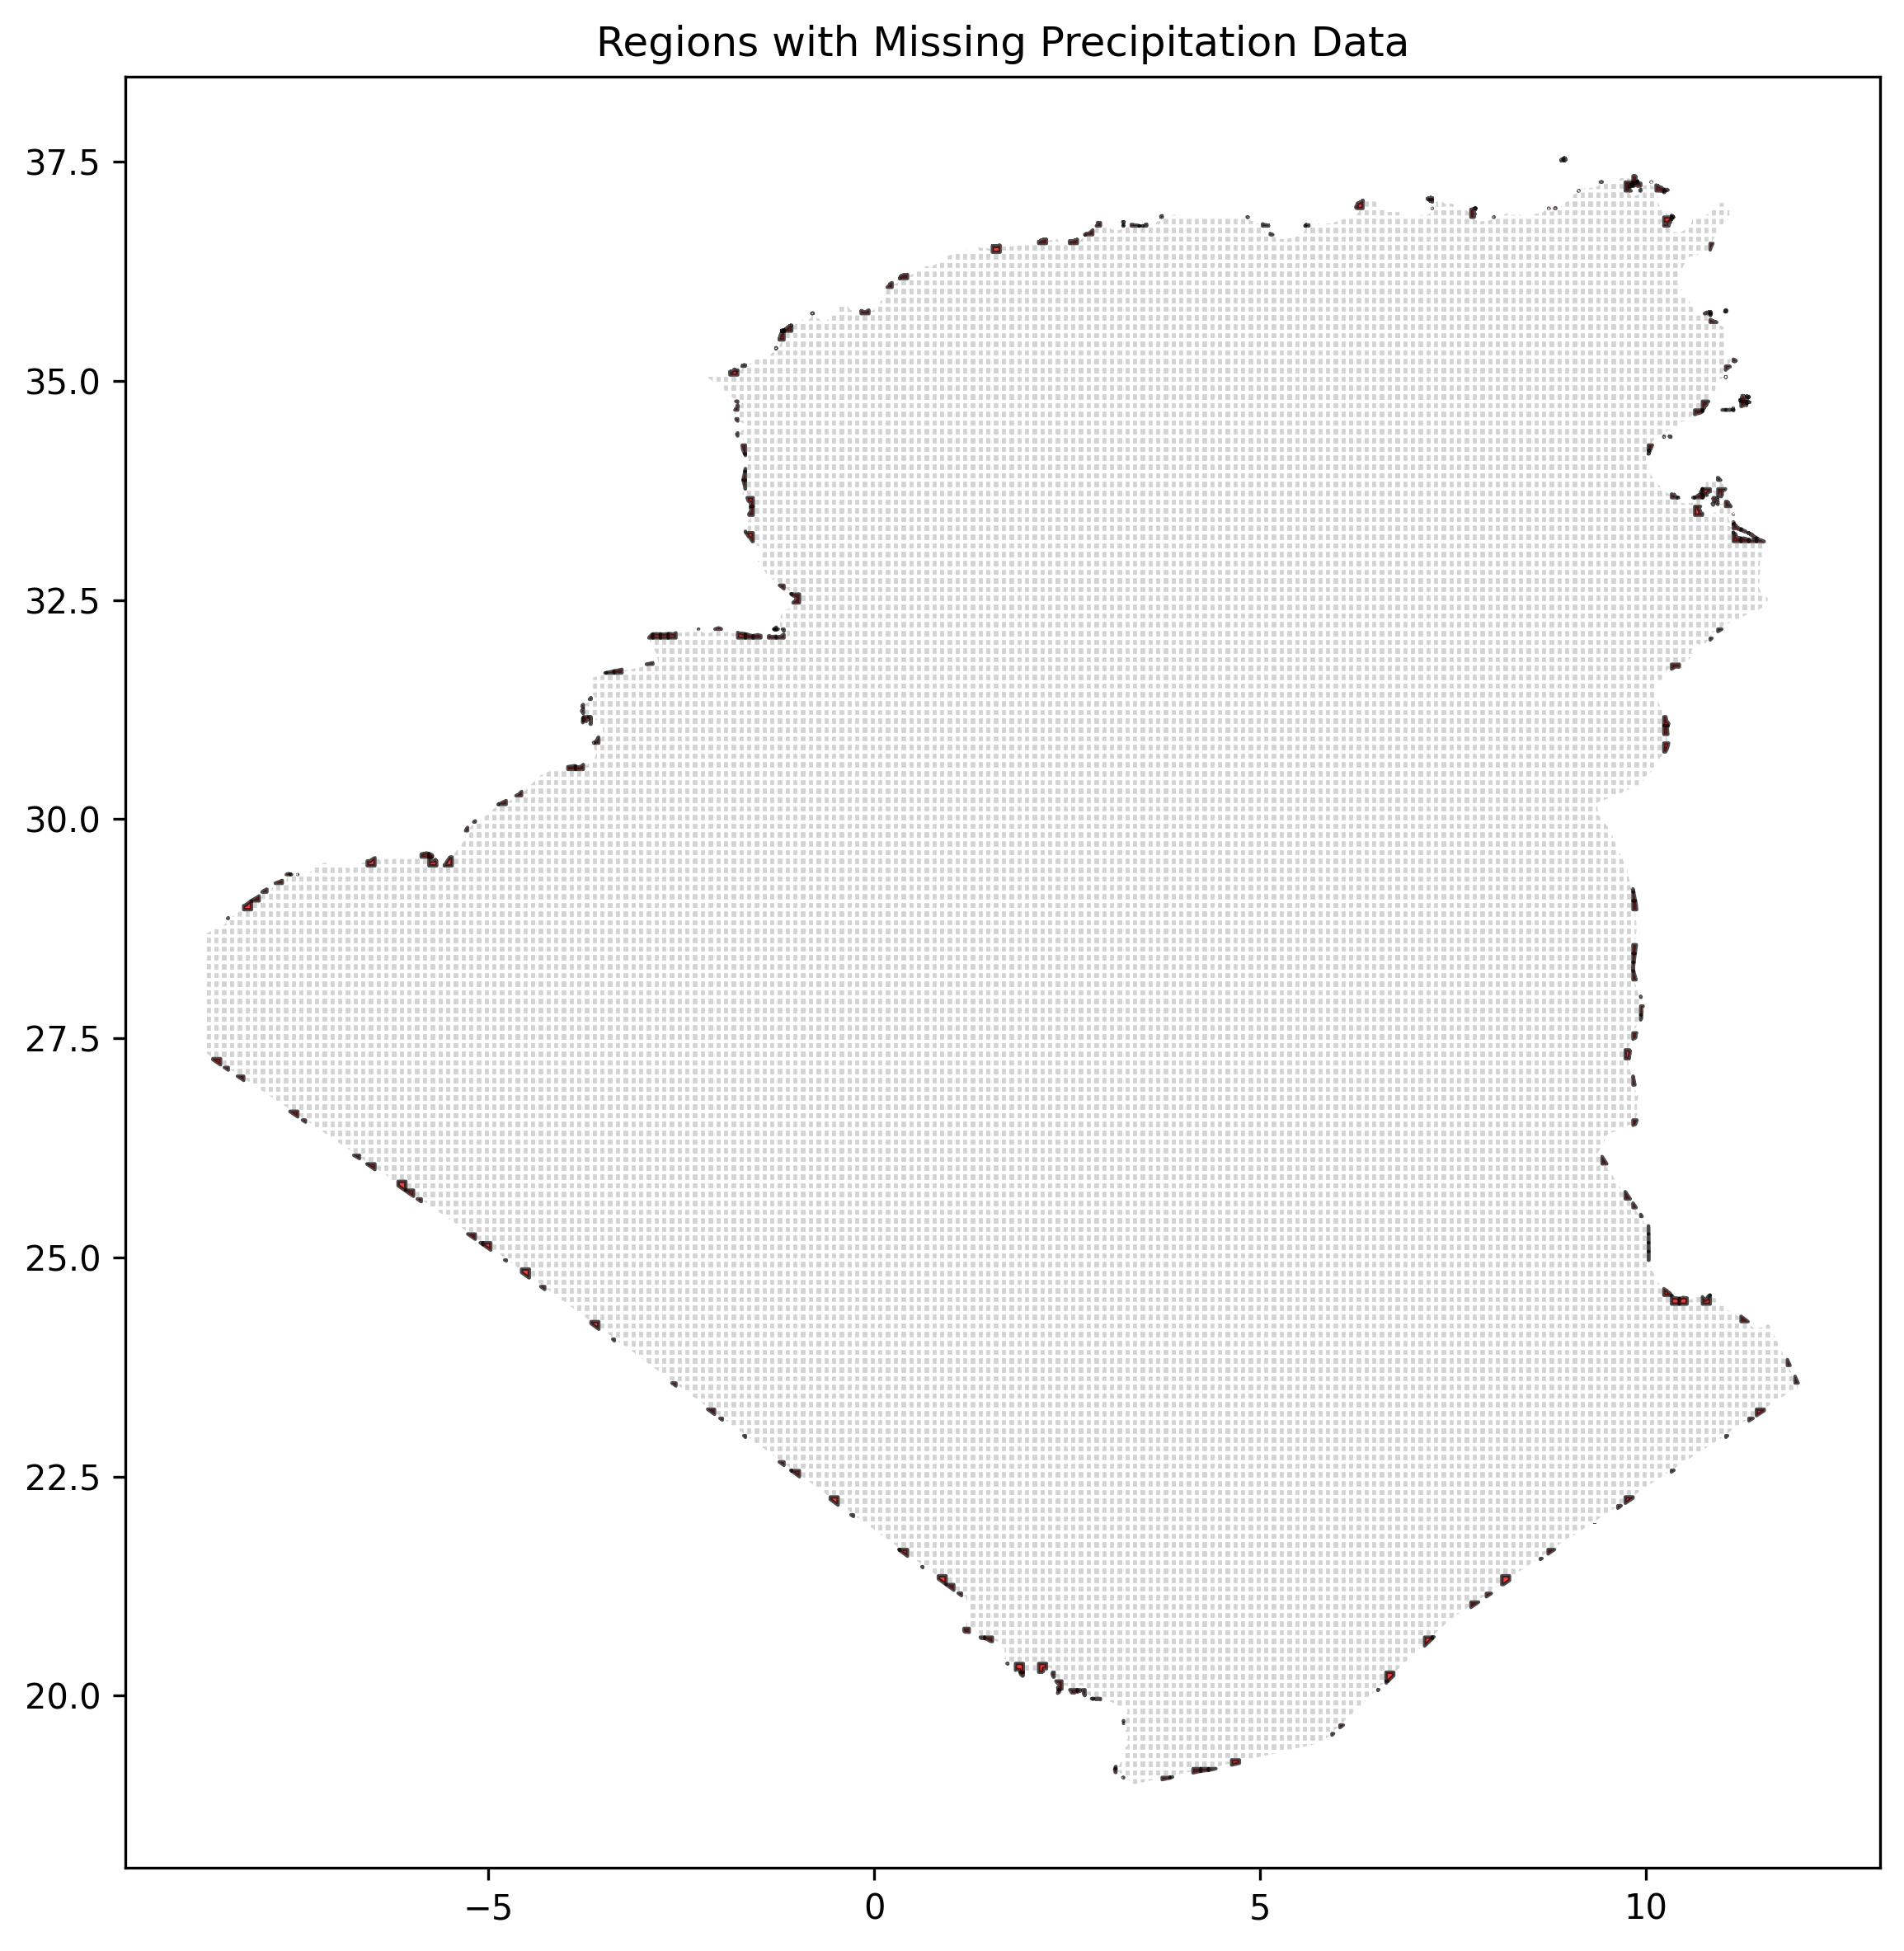
\includegraphics[width=\linewidth]{images/Climate/missing_precipitation_spatial.png}
\caption{Spatial distribution of missing precipitation values, concentrated along the AOI boundaries.}
\label{fig:missing_spatial}
\end{minipage}
\end{figure}


\subsection{Imputation Strategy}

To address missing values while preserving spatial coherence, a two-stage imputation strategy was adopted:
\begin{enumerate}
    \item \textbf{Primary KNN imputation}: Missing values were first imputed using a k-nearest neighbors approach based on spatial proximity, successfully filling approximately 77\% of missing entries.
    \item \textbf{Monthly climatology fallback}: Remaining missing values were imputed using the long-term monthly mean computed over all years for the corresponding variable and month.
\end{enumerate}

This approach ensures that local spatial structure is preserved whenever possible, while guaranteeing complete coverage when neighborhood-based imputation fails (e.g., at extreme boundaries).

After imputation, all missing values were fully resolved:
\[
\text{Precip missing} = 0,\quad \text{Tmax missing} = 0,\quad \text{Tmin missing} = 0.
\]

